\section[Desenvolvimento do Projeto]{Desenvolvimento do Projeto} 
Esta seção tem como objetivo detalhar as ferramentas escolhidas pela equipe para o desenvolvimento do projeto. Abaixo estão descritas as informações referentes ao repositório do código-fonte, o banco de dados utilizado, a arquitetura do sistema, os protótipos das telas e as tecnologias adotadas.

\subsection{Repositório do Código-Fonte do Projeto} 
O repositório responsável por armazenar e manter o controle de versão do código-fonte do projeto está disponível para consulta no seguinte link: 
\href{https://tools.ages.pucrs.br/meditamamente}{\textit{Repositório do Código Fonte}}

\subsection{Banco de Dados Utilizado}
O sistema de gerenciamento de banco de dados utilizado para armazenar os dados das atrações turísticas cadastradas e as informações dos contribuidores foi o MySQL \cite{MySQL}, um banco de dados relacional amplamente utilizado para gerenciar as informações dos usuários registrados no projeto. Mais detalhes podem ser encontrados clicando aqui:
\href{https://tools.ages.pucrs.br/meditamamente/wiki/-/wikis/database}{\textit{Banco de Dados}}

\begin{figure}[H]
    \centering
    \small
    \caption{Diagrama entidade-relacionamento do banco de dados do meditAMAmente}
    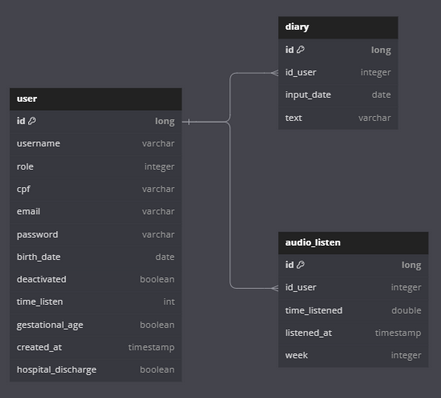
\includegraphics[width=0.7\linewidth]{conteudo/3 - ages II/conteudo/figures/bd_diagrama_entidade_relacionamento.png}\\
    \label{fig:medita-bd-er}
    \href{https://tools.ages.pucrs.br/meditamamente/wiki/-/wikis/database}{\textit{Fonte: https://tools.ages.pucrs.br/meditamamente/wiki/-/wikis/database}}
\end{figure}

\subsection{Arquitetura Utilizada}
A arquitetura do front-end é organizada em três principais diretórios: \textit{modules}, que contém as dependências instaladas via \textit{npm} ou \textit{yarn}; \textit{public}, onde ficam arquivos estáticos como imagens e fontes; e \textit{src}, que contém o código-fonte principal do projeto. Dentro do diretório \textit{src}, a pasta app é subdividida em outras pastas, cada uma responsável por diferentes aspectos do sistema, como tipagem, chamadas e configurações de APIs, além de armazenamento de componentes. Em conjunto com a cliente, optou-se por trocar a versão mobile do aplicativo por uma aplicação web responsiva, reduzindo os custos e facilitando o acesso via link, sem a necessidade de download. Mais informações sobre a arquitetura estão disponíveis em:
\href{https://tools.ages.pucrs.br/meditamamente/wiki/-/wikis/arquitetura}{\textit{Arquitetura}}

\begin{figure}[H]
    \centering
    \small
    \caption{Diagrama de \textit{deploy} da infraestrutura do meditAMAmente}
    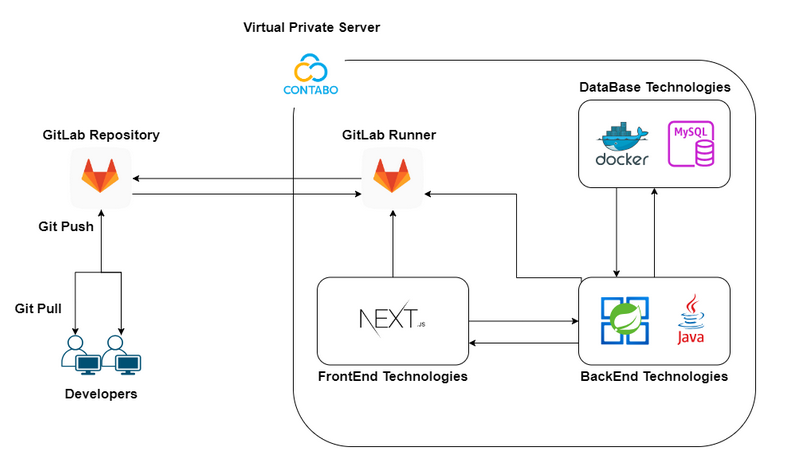
\includegraphics[width=0.9\linewidth]{conteudo/3 - ages II/conteudo/figures/diagrama_de_deploy.png}\\
    \label{fig:medita-diagrama-deploy}
    \href{https://tools.ages.pucrs.br/meditamamente/wiki/-/wikis/arquitetura}{\textit{Fonte: https://tools.ages.pucrs.br/meditamamente/wiki/-/wikis/arquitetura}}
\end{figure}

\subsection{Protótipos das Telas Desenvolvidas}
Os protótipos das telas foram criados utilizando a plataforma Figma. Os \textit{mockups} de cada tela podem ser visualizados no seguinte link:
\href{https://tools.ages.pucrs.br/meditamamente/wiki/-/wikis/mockups}{\textit{Protótipo das Telas}}

\begin{figure}[H]
    \centering
    \small
    \caption{Protótipos das telas de boas-vindas, login e inicial do aplicativo da mãe}
    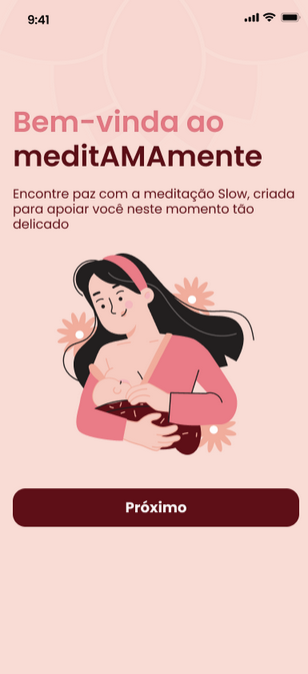
\includegraphics[width=0.31\linewidth]{conteudo/3 - ages II/conteudo/figures/tela_de_boas_vindas.png}\hfill
    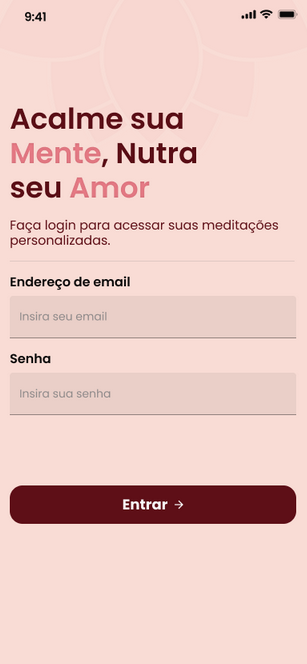
\includegraphics[width=0.31\linewidth]{conteudo/3 - ages II/conteudo/figures/tela_de_login.png}\hfill
    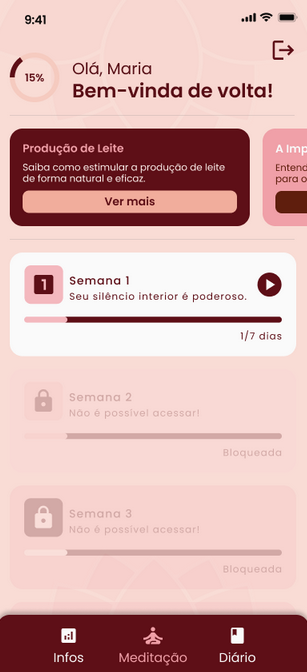
\includegraphics[width=0.31\linewidth]{conteudo/3 - ages II/conteudo/figures/tela_inicial.png}\\
    \label{fig:medita-mockups-mae}
    \href{https://tools.ages.pucrs.br/meditamamente/wiki/-/wikis/mockups}{\textit{Fonte: https://tools.ages.pucrs.br/meditamamente/wiki/-/wikis/mockups}}
\end{figure}

\begin{figure}[H]
    \centering
    \small
    \caption{Protótipos das telas de login e \textit{dashboard} do sistema web do pesquisador}
    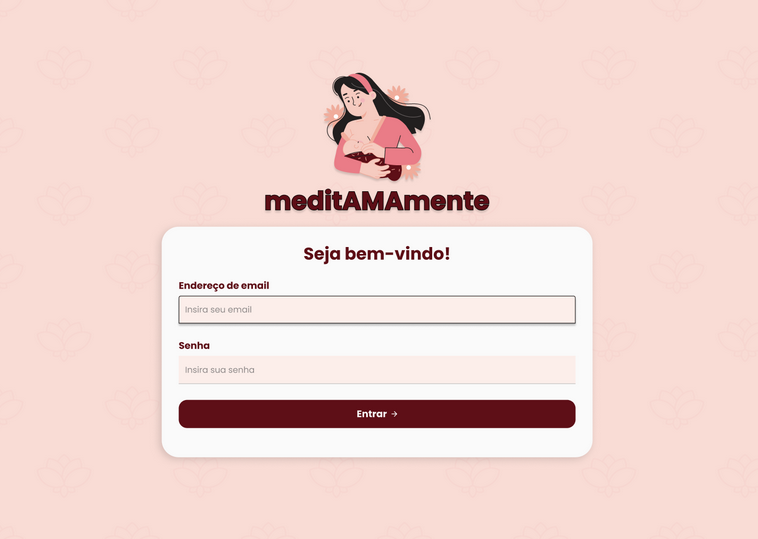
\includegraphics[width=0.45\linewidth]{conteudo/3 - ages II/conteudo/figures/tela_de_login_website.png}\hfill
    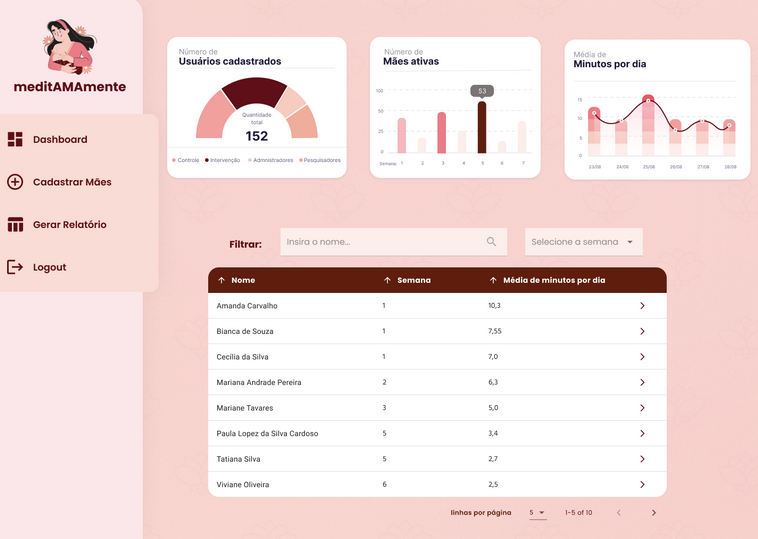
\includegraphics[width=0.45\linewidth]{conteudo/3 - ages II/conteudo/figures/tela_do_dashboard_website.png}\\
    \label{fig:medita-mockups-web}
    \href{https://tools.ages.pucrs.br/meditamamente/wiki/-/wikis/mockups}{\textit{Fonte: https://tools.ages.pucrs.br/meditamamente/wiki/-/wikis/mockups}}
\end{figure}

\subsection{Tecnologias Utilizadas}
Para o front-end, a equipe escolheu trabalhar com TypeScript \cite{Typescript} e o framework Next.js \cite{Next.js}. No back-end, o desenvolvimento foi feito em Java \cite{Java} com Spring Boot \cite{SpringBoot}. O banco de dados escolhido foi o MySQL, responsável por armazenar informações críticas do sistema, como os dados cadastrais das participantes, os diários escritos por elas, o cadastro de administradores, o armazenamento de áudios e a gestão de funcionalidades, conforme definido no projeto de extensão da cliente. Mais informações sobre as tecnologias podem ser encontradas no link:
\href{https://tools.ages.pucrs.br/meditamamente/wiki/-/wikis/arquitetura}{\textit{Tecnologias}}
